%%%%%%%%%%%%%%%%%%%%%%%%%%%%%%%%%%%%%%%%%
% University/School Laboratory Report
% LaTeX Template
% Version 3.1 (25/3/14)
%
% This template has been downloaded from:
% http://www.LaTeXTemplates.com
%
% Original author:
% Linux and Unix Users Group at Virginia Tech Wiki 
% (https://vtluug.org/wiki/Example_LaTeX_chem_lab_report)
%
% License:
% CC BY-NC-SA 3.0 (http://creativecommons.org/licenses/by-nc-sa/3.0/)
%
%%%%%%%%%%%%%%%%%%%%%%%%%%%%%%%%%%%%%%%%%

%----------------------------------------------------------------------------------------
%	PACKAGES AND DOCUMENT CONFIGURATIONS
%----------------------------------------------------------------------------------------

\documentclass{article}

\usepackage[version=3]{mhchem} % Package for chemical equation typesetting
\usepackage{siunitx} % Provides the \SI{}{} and \si{} command for typesetting SI units
\usepackage{graphicx} % Required for the inclusion of images
\usepackage{natbib} % Required to change bibliography style to APA
\usepackage{amsmath} % Required for some math elements 
%\usepackage{url}
\usepackage{hyperref}
\usepackage{subcaption}
\usepackage{float}
\usepackage{array}



\setlength\parindent{0pt} % Removes all indentation from paragraphs

%\renewcommand{\labelenumi}{\alph{enumi}.} % Make numbering in the enumerate environment by letter rather than number (e.g. section 6)

%\usepackage{times} % Uncomment to use the Times New Roman font

%----------------------------------------------------------------------------------------
%	DOCUMENT INFORMATION
%----------------------------------------------------------------------------------------

\title{Homework \#2 \\AES implementation \\[0.2em]\small{}CNS Course Sapienza} % Title and subtitle

\author{Riccardo \textsc{Prinzivalle}, 1904064} % Author name

\date{October 30, 2020} % Date for the report

\begin{document}

\maketitle % Insert the title, author and date

%----------------------------------------------------------------------------------------
%	SECTION 1
%----------------------------------------------------------------------------------------

\section{Homework Goal}

This homework contains a basic python implementation of AES algorithm. Throughout the work, it has been chosen to make a compromise: the implementation is in midpoint between complete Galois Field and precomputed look-up tables for every step. Both encryption and decryption are studied and implemented, then the operation modes are implemented and finally it will illustrate a comparison with world known AES implementation.

\section{Encryption}
Before digging into the details of every operation performed, it is necessary to explain how the variables are stored in this implementation: the 4x4 state matrix is treated as single vector of 16 components, from which of course it is possible to build the matrix representation and vice versa, it was only a choice due to initial lack of knowledge of python language; every state component is a byte stored in hex values to simplify computations (as I discovered python stores hex values as int so in practice the byte blocks are stored as int). Also the key is stored as an array of 16 bytes, and every byte follows the same philosophy adopted for the state. \newline
The encryption function is \textit{encrypt}, and it is composed by a sequence of the following four big blocks:  

\begin{enumerate}
\begin{item}
Byte Substitution
\end{item}
\begin{item}
Shift Row 
\end{item}
\begin{item}
Mix Columns
\end{item}
\begin{item}
Key Addition 
\end{item}
\end{enumerate}

The following subsections contain implementation details and choices made to build the single blocks.

\subsection{Byte Substitution}

The byte substitution block is build by two functions, one performs the single byte substitution operation (\textit {subByteSingle}), while the other one (\textit {subByte}) performs the byte substitution for all the bytes of the state calling the previous function for every single byte. The basic operation of single byte substitution is performed simply by looking to a prestored table which contains all the values for the 256 combinations of 8 bit contained in one byte. This method is more efficient and more simpler to implement with respect to performing all the operations needed in GF(256).

\subsection{Shift Row}

The shift row block is a simple function which perform a left row shift for every row of the state matrix; since the state is sorted as a plain array, it is necessary first to build the row of the matrix from the array, then performs the row shift and finally substitutes back in the state array the shifted value. As written in AES standard, the shift is of one byte more every time one new row is processed (first row has no shift while last row has a circular shift of 3 bytes). 

\subsection{Mix Columns}

The mix column block is based on an intermediate difficulty of implementation: the base idea is taken from \cite{10.5555/560131}, this idea is the core operation (fig. \ref{fig:core}) performed inside the \textit{mixcolumns} function. In order to perform it, it is necessary to construct the columns from the state array and in the end rebuild the state vector from the columns. The central operation is based on another function called \textit{xtime}, which together with the xor operations, is able to substitute all the GF operations. The \textit{xtime} function implements the multiplication of the polynomial stored in the byte times x, its idea is taken from \cite{AESxtime} and since the algorithm works with a byte implementation, it is necessary to use the final `and' in the return of the function to truncate the byte after the left shift. \newline
To debug this section, I used the test vectors which can be found in \cite{AESmixcolumn}.

\subsection{Key Addition}

The key addition layer basically uses 3 functions in this implementation: \textit{keyAddition} performs the xor operation between the state and the subkey (the for is necessary to perform the operation bytewise, since the state is an array); \textit{roundKey} generates the subkeys needed at every iteration of AES while \textit{gFunction} is an auxiliary function needed by \textit{roundKey}. \newline
The \textit{gFunction} corresponds to function \textit{g} of classical AES implementation, the shift and the byte substitution are based on previous functions or parts of them, while the xor operation is performed with a precomputed vector instead of computing at every round the specific byte to xor. In this way, the implementation is more efficient and simpler.\newline
The \textit{roundKey} function first joins 4 bytes of the key at a time in order to work with words, then it needs the auxiliary \textit{gFunction}, then it performs the four cascaded xor and finally it rebuilds the byte based key from the words.\newline
To debug this section, it has been used a step by step subkey generation that can be found in \cite{AESsteps}.   

%----------------------------------------------------------------------------------------
%	SECTION 2
%----------------------------------------------------------------------------------------

\section{Decryption}

The decryption part of AES is simpler than encryption since it is possible to reuse at least the key addition layer; based on implementation choices, as those made in this work, it is possible to reuse also the \textit{mixcolumn} idea in its inverse. The decryption is less efficient than its counterpart since it generates the subkeys at every round instead of generating it once and storing it, this has been chosen to speed up the implementation. The decryption function is called \textit{decrypt}.
 
\subsection{Mix Columns Inverse}

The inverse of \textit{mixcolumns} reuses part of its direct function together with a precomputation: the columns are preprocessed (fig. \ref{fig:preprocessing}) and then they are elaborated by the \textit{mixcolumns} core (fig. \ref{fig:core}). All the mathematical details on this choice can be found in chapter 4 of \cite{10.5555/560131}. 

\begin{figure}[H]
\centering
\begin{subfigure}{.54\textwidth}
  \centering
  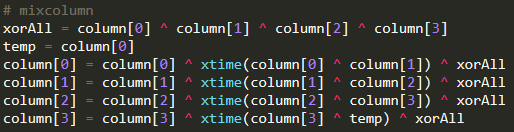
\includegraphics[width=1\linewidth]{images/mixcolumn.png}
  \caption{Core}
  \label{fig:core}
\end{subfigure}
\begin{subfigure}{.35\textwidth}
  \centering
  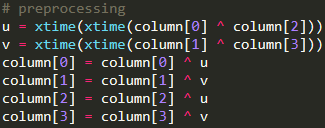
\includegraphics[width=1\linewidth]{images/preprocessing.png}
  \caption{Preprocessing}
  \label{fig:preprocessing}
\end{subfigure}
\caption{Mix columns base functions}
\label{fig:MixColumns}
\end{figure}

\subsection{Shift Row Inverse}

This block performs the row shift to the right, in order to reverse the \textit{shiftRow} operation. As before, from state it builds the necessary rows and at the end the state is rebuilt from each rows. In order to reverse the direct operation, the first row is not shifted while the others receive successive shift till the third row which undergoes a right shift of three elements.

\subsection{Byte Substitution Inverse}

This layer performs the inverse operation of Byte Substitution; it is based on two functions: \textit{subByteInv} is just a wrapper to call the base function on every byte of the state; \textit{subByteSingleInv} instead is the base function which performs the inverse Byte Substitution based on the inverse table seen before in the \textit{subByteSingle}.
 
%----------------------------------------------------------------------------------------
%	SECTION 3
%----------------------------------------------------------------------------------------

\section{Operation Modes}

Operation modes allows to use a block cipher as AES in the case the message has length different from one block size: in this case, it is possible to encrypt multiple blocks or even deal with blocks of length different from 128 bit. In order to work with different blocks, we need to manipulate the input: in this work, it is assumed to receive a string of hex numbers as input, as in table \ref{tab:AESparameter}, so it is necessary to have some input manipulation function.\newline
The values in table \ref{tab:AESparameter} are taken from example of implementation of AES found on GitHub.

\begin{table}[H]
\begin{center}
\begin{tabular}{ll}
Input text &  6bc1bee22e409f96e93d7e117393172a\\
	      &   ae2d8a571e03ac9c9eb76fac45af8e51\\
	      &   30c81c46a35ce411e5fbc1191a0a52ef\\
	      &   f69f2445df4f9b17ad2b417be66c37 \\
\\
Key & 2b7e151628aed2a6abf7158809cf4f3c\\
\\
IV (where needed) & 5468617473206D79204B756E67204675
\end{tabular}
\caption{Parameter used in testing of AES operation modes}
\label{tab:AESparameter}
\end{center}
\end{table}

\subsection{Text to Blocks}

First it is necessary the \textit{text2blocks} function, which divides the hex string received as input into the blocks that can be encrypted by AES. In this step a problem arises: what to do with blocks whose length is different from block size? It has been chosen in this work to use the padding scheme PKCS\#7, which in this case added a number of bytes to complete the block with value equal to the number of missing bytes; in the special case when the last block has length equal to block size, the padding scheme plans to add a new block composed by bytes whose value is equal to block size in bytes (16 in this case so a block composed by 10 in hex base). The padding is added during text to block conversion by a similar function as those explained before, the only difference is that it adds padding to the last block; this function is \textit{text2blocksPadding}. To have a better understanding of why it was necessary to design two similar functions, there it is their main motivation: \textit{text2blocksPadding} is used with plaintext as input, so it must add padding since text is going to be transformed and aligned to block dimension; \textit{text2blocks} is used in decryption with ciphertext as input, so the padding has already been added in encryption and it is necessary to just split the text into blocks whose length is exactly equal to block size.

\subsection{Blocks to Text}

To obtain the text from an array of blocks, some extra functions are needed: \textit{blocks2text} and \textit{blocks2textPadding}, whose aim is the inverse of that of previous section. The first is used at the end of encryption phase to obtain the ciphertext from the array of encrypted blocks. Special mention goes to the second function, which works at the end of decryption to join plain blocks into the decrypted plaintext: in this case it is necessary to reverse and remove the padding scheme used, this operation is simpler when the last byte of last block is 16 in base ten since we simply remove the last block from the the array (and the corresponding list made to host the blocks undergoing manipulation); in the case the last byte read is different from 16, it is necessary to remove a number of couples (every byte is in hex, so two cipher must be removed) equal to the last byte read and this is done by a simple iterative \textit{pop}. 

\subsection{Block manipulation}

Since the state is a list of 16 int representing the 16 bytes, it is necessary to transform every block (which contains a string of hex values) into the int array needed by encryption function: this operation is performed by \textit{block2int} function. The reverse function, \textit{int2block}, allows to recover the block string from the list of 16 int which was used as state.  

\subsection{Implementation notes}

All the operation modes have been implemented based on the slide of the course, CBC and CFB cause some problems since the following block to be encrypted needs to know the previous encrypted block, and due to the different implementation of \textit{block2int} and \textit{int2block}, it is necessary from the second block on to delete the spaces the function \textit{int2block} introduces in order to have the right input for \textit{block2int} in the following block computations.
\newline
Another problem is in the CTR, since for every block it is needed to increment the nonce, and a problem may arise when the increment arrives to the byte in position 0 in the block array and the current value is 255, I am not able to decide what to do in this situation, so I used a nonce which does not create this problem in the test (I know this is not the right way to do it). Furthermore, this implementation uses a 128 bit nonce; this is because initially I wasn't able to find a standard and I thought the nonce was all the 128 bit and it is incremented; then I found that \textit{pycryptodome}, the library chosen as standard for the comparison, implemented a 64 bit nonce plus a 64 bit counter and they are put one at the side of the other to build a 128 bit IV. Both these standard are documented in \cite{NIST}, so I had chosen to stay firm in my choice, so experimental result will be different. Perhaps, on further digging on the net, I found that it is possible to use an IV of 128 bit where the left 96 bits are nonce and the remaining 32 bits on the right are dedicated to counter, this is specified in \cite{stack}.
\newline
Instead, ECB and OFB were simpler to implement due to their simpler algorithm.
\newline
A note on the implementation of CFB: it can be implemented choosing a variable number of bits of ciphertext to xor in the following iteration, in this case, to simplify the implementation, it has been chosen to xor the complete block. 



%----------------------------------------------------------------------------------------
%	SECTION 4
%----------------------------------------------------------------------------------------

\section{Real World Standard Comparison}

As validation and comparison of the implementation in this report, it has been chosen \textit{PyCryptoDome} as test library. 

\subsection{Validation}

All the operation modes asked in the homework are available in \textit{PyCryptoDome}, so as an initial validation all operational modes are implemented. To have a fair comparison, the padding scheme is added manually in the case of library test in order to obtain also the last block equal to the implementation proposed. 

\begin{figure}[H]
\centering
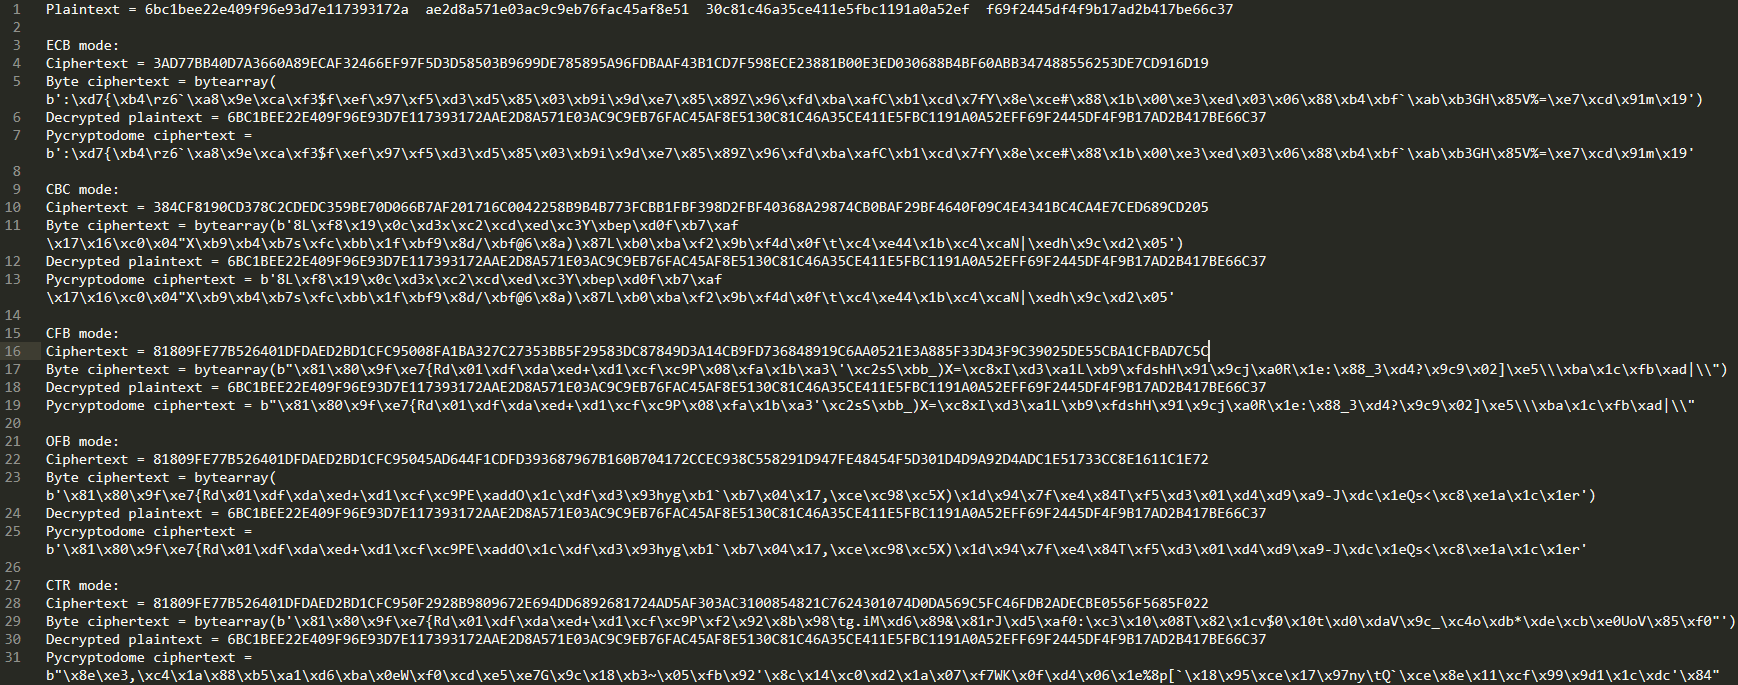
\includegraphics[width=1\linewidth]{images/output_comparison.png}
\caption{Output comparison with  \textit{PyCryptoDome}}
\label{fig:outputComparison}
\end{figure}

As it is possible to see in Fig. \ref{fig:outputComparison}, the first four operation modes gives the same result as the implementation proposed, while the last mode, which is CTR, gives a different result since the nonce vector in \textit{PyCryptoDome} library is only of 64 bit and the remaining 64 bits of IV are dedicated to counter, while in the implementation proposed the nonce and counter are brought together in a 128 bit vector.

\subsection{Throughput Comparison}

To have a fair comparison, the implementation proposed has been tested together with the \textit{PyCryptoDome} library on 3 files of fixed dimensions: 1KB, 100KB and 10MB. The code for file processing is based on \cite{pycryptodome}. As specified on the request, only 3 operation modes are tested, in this case it has been chosen to use ECB, OFB and CBC. To optimize time, the test are run a different number of times: the 1KB file test is run 100 times, the 100KB is run 10 times and the 10MB test is run 5 times only, since the proposed implementation requires around 40 minutes to run the most intensive test.
\newline
The most efficient encryption implementation is ECB, which needs around 20 minutes to encrypt the 10MB files 5 times, it results in a medium time of 3.79 minutes and a throughput of 45KB/s; the other have smaller but similar throughput: 44.5KB/s for OFB and 43.6KB/s for CBC. These values were computed in the case of 10MB file. The other encryption throughputs can be seen in table \ref{tab:enc}.

\renewcommand{\arraystretch}{2}

\begin{table}[H]
\begin{center}
\begin{tabular}{ |c || m{2cm} | m{2cm} | m{2cm}|  }
\hline
  Encryption & 1KB & 100KB & 10MB \\ [0.5ex] 
 \hline\hline
   ECB & 45,22 KB/s & 45,17 KB/s & 45 KB/s \\ 
 \hline
  ECB PyCryptoDome & 7,5 MB/s & 325 MB/s & 714 MB/s \\ 
 \hline
 OFB & 44,04 KB/s & 44,28 KB/s &  44,5 KB/s \\
 \hline
  OFB PyCryptoDome & 6,97 MB/s & 244,1 MB/s &  433,92 MB/s \\
 \hline
 CBC & 43,20 KB/s & 43,42 KB/s &  43,6 KB/s \\ 
 \hline
  CBC PyCryptoDome & 6,96 MB/s & 195,28 MB/s &  442,49 MB/s \\
 \hline
\end{tabular}
\caption{AES encryption throughput}
\label{tab:enc}
\end{center}
\end{table}

As seen in table \ref{tab:enc}, the library implementation is much more faster. That is normal since the library has undergone different improvements during its development. There's a thing in \textit{PyCryptoDome} library that astonish me: growing the file dimension, also the throughput increases. Similar comparison happens in the decryption phase as shown in table \ref{tab:dec}; in this case it is expected a lower throughput since the decryption function is less optimized and it wastes computational time not storing the subkeys but computing them in every round.

\begin{table}[h]
\begin{center}
\begin{tabular}{ | c || m{2cm} | m{2cm} | m{2cm}|  }
\hline
  Decryption & 1KB & 100KB & 10MB \\ [0.5ex] 
 \hline\hline
   ECB & 22,14 KB/s & 22,3 KB/s & 22,287 KB/s \\ 
 \hline
  ECB PyCryptoDome & 7,5 MB/s & 488 MB/s & 2,12 GB/s \\ 
 \hline
 OFB & 44,61 KB/s & 45,05 KB/s &  45,26 KB/s \\
 \hline
  OFB PyCryptoDome & 6,95 MB/s & 244,07 MB/s &  454,4 MB/s \\
 \hline
 CBC & 22,01 KB/s & 22,23 KB/s &  22,43 KB/s \\ 
 \hline
  CBC PyCryptoDome & 6,97 MB/s & 244,08 MB/s &  480,66 MB/s \\
 \hline
\end{tabular}
\caption{Implemented AES decryption throughput}
\label{tab:dec}
\end{center}
\end{table}

The implementation proposed has a strange behavior in decryption: while in encryption the three modes chosen present at maximum a difference of 2 KB/s, in decryption the OFB is the only one having performances in line with encryption, while the other two modes has more or less half of the performance with respect to their counterpart in encryption.

%----------------------------------------------------------------------------------------
%	SECTION 5
%----------------------------------------------------------------------------------------

\section{Conclusion}

Even if the implementation proposed is much slower than the standard library chosen as comparison, it works well and it does its dirty job. The code may not be much optimized or it can have been written in a better way but my knowledge in python is not so huge, but this was an opportunity to dust and improve my experience.


%----------------------------------------------------------------------------------------
%	BIBLIOGRAPHY
%----------------------------------------------------------------------------------------

\bibliographystyle{abbrv}

\bibliography{sample}

%----------------------------------------------------------------------------------------


\end{document}